%\subsection{Introduction}\label{in/troduction}

This section delves into the fundamental mechanisms that underpin the
operation of decentralized networks: consensus protocols. These
protocols are the cornerstone of any blockchain, as they provide the
means for a distributed network of independent and potentially
untrusting nodes to reach an agreement on the state of the ledger. As we
will learn, achieving this ``agreement'' or ``consensus'' in a
decentralized environment is a non-trivial challenge, especially when
considering the potential for network delays, failures, and even
malicious participants.

We will begin by exploring the theoretical foundations of consensus,
including the different types of blockchain networks and how they manage
access and participation. We will dissect the inherent trade-offs in
distributed systems as encapsulated by the famous CAP theorem, and
understand why blockchains must often prioritize availability and
partition tolerance, leading to a model of ``eventual consistency.'' We
will also define the critical properties that a robust consensus
protocol must satisfy -- namely \textbf{safety, liveness, and finality} -- to
ensure the network remains secure and functional.

The section will then proceed to examine the two primary paradigms for
achieving consensus: \textbf{lottery-based} and \textbf{voting-based} mechanisms. We will
analyze the respective strengths and weaknesses of each approach,
considering factors such as scalability, network overhead, and the time
it takes for transactions to be irreversibly confirmed. A significant
portion of the section will be dedicated to understanding the concept of
\textbf{forks} -- a natural consequence of the probabilistic nature of some
consensus protocols -- and the mechanisms used to resolve them.

Furthermore, we will explore the classic \textbf{Byzantine Generals Problem},
which provides a powerful analogy for understanding the challenges of
achieving consensus in the presence of malicious actors. This will lead
to a discussion of Byzantine Fault Tolerance (BFT) and its practical
implementation in the form of the Practical Byzantine Fault Tolerance
(PBFT) algorithm, a protocol foundational to many permissioned
blockchains.

Finally, we will examine the most prominent consensus protocols used in
practice today. This includes Proof-of-Work (PoW), the original,
resource-intensive mechanism of Bitcoin; Proof-of-Stake (PoS), a more
energy-efficient alternative that has been adopted by many modern
blockchains like Ethereum; and \textbf{Proof-of-Authority} (PoA), a
reputation-based mechanism well-suited for private, permissioned
networks. We will also discuss the crucial role of incentive schemes in
securing permissionless networks and the complex challenges of managing
decentralized names and identities.

\subsection{Learning Objectives}\label{learning-objectives}

\begin{itemize}
	\tightlist
	\item
	Understand the different types of blockchain networks (permissionless,
	permissioned, and semi-permissionless) and their methods for
	controlling entry and preventing Sybil attacks.
	\item
	Grasp the concepts of the CAP theorem and its implications for
	blockchain design, particularly the trade-off between consistency and
	availability.
	\item
	Learn the standard goals of consensus protocols: safety (agreement),
	liveness (termination), and finality (eventual consistency).
	\item
	Differentiate between lottery-based and voting-based consensus
	mechanisms and their respective trade-offs.
	\item
	Understand the concept of forks (accidental, malicious, and
	intentional) and the fork-choice rules used to resolve them.
	\item
	Gain insight into the Byzantine Generals Problem and its relevance to
	fault tolerance in distributed systems.
	\item
	Learn about specific consensus protocols, including Practical
	Byzantine Fault Tolerance (PBFT), Proof-of-Work (PoW), and
	Proof-of-Stake (PoS).
	\item
	Understand the role of incentive schemes in motivating honest
	participation in blockchain networks.
	\item
	Understand the challenges of decentralized identity management as
	described by Zooko's Triangle.
\end{itemize}

\begin{center}\rule{0.5\linewidth}{0.5pt}\end{center}

\subsection{Blockchain Networks and System
	Models}\label{section-1-blockchain-networks-and-system-models}

\subsubsection{Types of Blockchains}\label{types-of-blockchains}

Blockchains can be broadly classified into three categories based on
their access control mechanisms, which determine how new nodes can join
the network and participate in the consensus process.

\begin{itemize}
	\item
	\textbf{Permissionless Blockchains}: These are open networks that
	anyone can join without requiring permission from a central authority.
	The core challenge in such a system is the \textbf{Sybil attack},
	where an attacker could create a large number of pseudonymous
	identities to gain a disproportionate influence on the network. 
%	As the 	lecturer explained, 
	If consensus were to be based on a simple vote, one
	could ``create a thousand fake identities and have a thousand votes.''
	To prevent this, permissionless blockchains employ
	\textbf{Proof-of-Resource} mechanisms. These mechanisms require nodes
	to demonstrate ownership of a scarce resource, such as computational
	power (in Proof-of-Work) or a significant financial stake (in
	Proof-of-Stake). A node's influence in the consensus process is
	directly proportional to the amount of the scarce resource it
	controls, not the number of identities it possesses. Bitcoin and
	Ethereum are prominent examples of permissionless blockchains.
	\item
	\textbf{Permissioned Blockchains}: In contrast to permissionless
	blockchains, these are closed networks where new nodes must obtain
	explicit permission to join from a centralized or federated authority.
	This authority is responsible for vetting and onboarding new
	participants. For instance, a bank operating its own blockchain would
	only allow vetted entities to join. Because participants are known and
	there's a mechanism to expel malicious actors, the risk of Sybil
	attacks is eliminated. This allows permissioned blockchains to use
	more traditional and efficient voting-based consensus protocols, such
	as Practical Byzantine Fault Tolerance (PBFT), where each node
	typically has an equal say (``one node, one vote''). These networks
	are well-suited for enterprise applications where privacy, control,
	and performance are paramount.
	\item
	\textbf{Semi-Permissionless Blockchains}: This category represents a
	hybrid approach, analogous to a joint-stock company where voting power
	is tied to ownership. While new nodes do not require permission from a
	central authority to join, they must acquire a ``stake'' in the
	network to participate in the consensus process. This stake, which is
	typically in the form of the network's native cryptocurrency, can be
	acquired from any existing participant. A node's consensus power is
	proportional to the size of its stake, which serves as a form of
	collateral that can be forfeited in the event of malicious behavior.
	This model aims to strike a balance between the openness of
	permissionless networks and the control of permissioned networks.
\end{itemize}

\subsubsection{Centralized vs.~Decentralized
	Systems}\label{centralized-vs.-decentralized-systems}

In the discourse surrounding blockchain technology, the terms
``distributed'' and ``decentralized'' are often used interchangeably,
but they refer to distinct concepts. A clear understanding of this
distinction is essential for appreciating the unique value proposition
of blockchains.

\begin{itemize}
	\item
	\textbf{Distributed Systems}: A distributed system (see \autoref{fig:distrib-decentralized}) is one in which
	components are located on different networked computers, which then
	communicate and coordinate their actions. The key characteristic of a
	distributed system is its \textbf{geographical distribution}. For
	example, a company like Google operates a massive distributed system
	with data centers located all over the world. However, despite its
	distributed nature, this system is still \textbf{centrally controlled}
	by a single entity.
	\item
	\textbf{Decentralized Systems}: A decentralized system, on the other
	hand, is defined by its \textbf{control and trust model}. In a fully
	decentralized system, there is no single point of control or trust.
	Instead, control is distributed among the participants, and decisions
	are made through a consensus mechanism. This eliminates the need for a
	trusted third party, as the system is designed to be resilient to the
	failure or malicious behavior of individual nodes.
\end{itemize}

While all decentralized systems are necessarily distributed, the
converse is not true. A system can be geographically distributed but
still be centrally controlled. The true innovation of blockchain
technology lies in its ability to create a fully decentralized system
that can operate in a trustless environment.

\begin{figure}[t]
	%	\vspace{-0.3cm}
	\begin{center}
		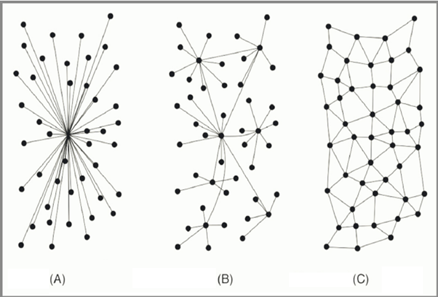
\includegraphics[width=0.8\textwidth]{./figs/distrib-decentralized.png} 
		\caption{(A) centralized system, (B) partially decentralized system, (C) fully decentralized system.}		
		\label{fig:distrib-decentralized}
	\end{center}	
\end{figure}

\subsubsection{The CAP Theorem}\label{the-cap-theorem}

The CAP theorem, also known as Brewer's theorem, is a fundamental
principle in distributed systems that describes an inherent trade-off
between three desirable properties: consistency, availability, and
partition tolerance. The theorem states that any distributed data store
can only provide two of these three guarantees simultaneously.

\begin{itemize}
	\tightlist
	\item
	\textbf{Consistency}: This guarantee ensures that all nodes in the
	network see the same data at the same time. In a consistent system,
	every read operation will return the value of the most recent write
	operation or an error.
	\item
	\textbf{Availability}: This guarantee ensures that every request to
	the system receives a response, without the guarantee that it contains
	the most recent write. In an available system, there are no single
	points of failure, and the system remains operational even if some
	nodes are down.
	\item
	\textbf{Partition Tolerance}: This guarantee ensures that the system
	continues to operate even if the network is partitioned, meaning that
	messages between nodes are dropped or delayed.
\end{itemize}

In the context of blockchain technology, which operates over the public
internet, network partitions are an unavoidable reality. Therefore, any
blockchain protocol \textbf{must be partition tolerant}. This leaves a
fundamental choice between consistency and availability.
%
Most blockchain protocols, particularly those based on Nakamoto
consensus, prioritize \textbf{availability and partition tolerance} over
strong consistency. This means that they will continue to operate and
process transactions even in the presence of network partitions, but at
the cost of immediate consistency. Instead, they offer a weaker form of
consistency known as \textbf{eventual consistency}. This means that
while different nodes may have a different view of the ledger at any
given moment, they will eventually converge on a single, consistent
state over time. This is typically achieved by requiring a certain
number of \textbf{confirmations} (i.e., subsequent blocks) before a
transaction is considered final. For example, in Bitcoin, a transaction
is conventionally considered secure and final after six confirmations,
which takes approximately 60 minutes.

\begin{figure}[t]
	%	\vspace{-0.3cm}
	\begin{center}
		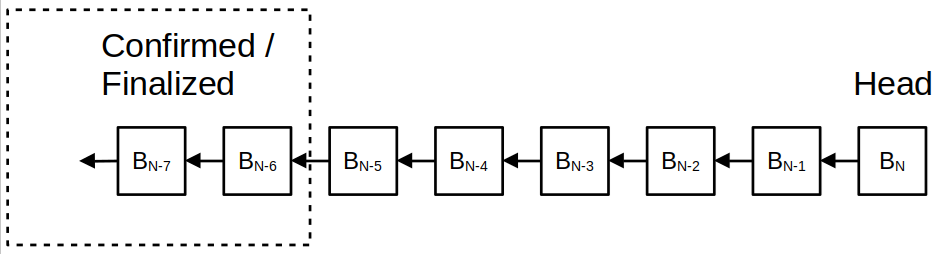
\includegraphics[width=0.8\textwidth]{./figs/btc-finality.png} 
		\caption{Eventual consistency of availability-favored blockchains within CAP theorem.}		
		\label{fig:btc-finality}
	\end{center}	
\end{figure}

\begin{center}\rule{0.5\linewidth}{0.5pt}\end{center}

\subsection{Consensus Protocols in
	Blockchains}\label{section-2-consensus-protocols-in-blockchains}

\subsubsection{Goals of Consensus
	Protocols}\label{goals-of-consensus-protocols}

Consensus protocols are the mechanisms by which a distributed network of
nodes can agree on a single, consistent history of transactions. These
protocols are designed to achieve several key goals, which are essential
for the secure and reliable operation of a blockchain.

\begin{itemize}
	\item
	\textbf{Safety (Agreement)}: This property ensures that all honest
	nodes in the network will eventually agree on the same value. In the
	context of a blockchain, this means that all honest nodes will have an
	identical copy of the ledger. Safety is a critical property, as it
	prevents a ``split-brain'' scenario where different parts of the
	network have conflicting views of the truth.
	\item
	\textbf{Liveness (Termination)}: This property ensures that the
	network will continue to make progress. In other words, all honest
	nodes will eventually decide on a value, and the blockchain does not
	stall. This ensures that new transactions are eventually included in
	the ledger.
	\item
	\textbf{Finality}: This is a concept that reinterprets safety and
	liveness in the context of blockchains that provide eventual
	consistency. A block is said to have reached finality when it is
	computationally infeasible for it to be overturned or removed from the
	blockchain (see \autoref{fig:btc-finality}). The time to finality can vary significantly between
	different consensus protocols. For example, in Bitcoin, a block is
	typically considered final after six subsequent blocks have been added
	to the chain, which takes approximately one hour. In contrast, some
	voting-based protocols can achieve finality in a matter of seconds.
\end{itemize}

\subsubsection{Lottery vs.~Voting}\label{lottery-vs.-voting}

At a high level, consensus protocols can be categorized into two main
approaches: lottery-based and voting-based~\cite{hyperledger1}.

\begin{itemize}
	\item
	\textbf{Lottery-Based Consensus}: In this approach, a single node is
	selected through a lottery-like mechanism to be the leader for a given
	round. This leader is then responsible for producing the next block
	and broadcasting it to the network. The probability of being selected
	as the leader is typically proportional to the amount of a scarce
	resource that a node controls, such as computational power in
	Proof-of-Work or stake in Proof-of-Stake. Lottery-based protocols are
	characterized by their low network overhead and high scalability, as
	they do not require all nodes to communicate with each other. However,
	they are susceptible to forks, which can occur if multiple leaders are
	elected simultaneously and propose conflicting blocks.
	\item
	\textbf{Voting-Based Consensus}: In this approach, all nodes in the
	network participate in a collective voting process to agree on the
	next block. This typically involves multiple rounds of communication,
	where nodes exchange messages to reach a consensus. Voting-based
	protocols, such as PBFT, offer the advantage of low-latency finality,
	as a block is considered final once it has been approved by a
	sufficient number of nodes. However, they suffer from high
	communication complexity, which is typically on the order of
	$O(N^2)$, where $N$ is the number of nodes. This makes them unsuitable
	for large, permissionless networks, but well-suited for smaller,
	permissioned blockchains where the number of participants is limited.
\end{itemize}

Many modern protocols, like Algorand~\cite{gilad2017algorand}, use a combination of these two
approaches, using a lottery to select a small committee of nodes which
then vote on the next block.

\subsubsection{Forks}\label{forks}

A fork is a situation where a blockchain diverges into two or more
competing chains. This can happen for a variety of reasons, and it is a
fundamental concept to understand in the context of blockchain
technology.

\begin{itemize}
	\item
	\textbf{Accidental Forks}: These are a natural consequence of the
	probabilistic nature of lottery-based consensus protocols. Due to
	network latency, it is possible for two or more nodes to solve the
	consensus puzzle at approximately the same time and broadcast their
	new blocks to the network. This can result in a temporary fork, where
	different parts of the network have a different view of the latest
	block. These forks are typically resolved quickly as subsequent blocks
	are added to one of the chains, making it the longest and therefore
	the canonical chain.
	\item
	\textbf{Malicious Forks}: These are intentionally created by attackers
	with the aim of disrupting the network or defrauding other users. A
	common example is a \textbf{double-spending attack}, where an attacker
	sends a transaction to a merchant, waits for the merchant to deliver
	the goods, and then creates a fork to reverse the transaction. Another
	example is \textbf{selfish mining}, where a miner with significant
	hash power secretly builds a longer chain and then releases it to the
	network to orphan the blocks of other miners and claim their rewards.
	\item
	\textbf{Intentional Forks (Hard Forks and Soft Forks)}: These are
	planned forks that are created to introduce changes to the protocol.
	
	\begin{itemize}
		\tightlist
		\item
		A \textbf{hard fork} is a backward-incompatible change to the
		protocol, which requires all nodes to upgrade to the new version. If
		some nodes do not upgrade, the blockchain will permanently split
		into two separate chains. The creation of Bitcoin Cash from Bitcoin,
		which increased the block size limit, is a well-known example of a
		hard fork.
		\item
		A \textbf{soft fork} is a backward-compatible change, which allows
		non-upgraded nodes to continue to participate in the network.
	\end{itemize}
\end{itemize}

Forks are typically resolved through a \textbf{fork-choice rule}, which
is a set of rules that nodes use to determine which chain to consider
the canonical one. The most common fork-choice rule is the
\textbf{longest chain rule}, which states that the valid chain is the
one with the most blocks (see \autoref{fig:longest-chain}), as it represents the most accumulated work.
Another approach is the \textbf{strongest chain rule}, which takes into
account the ``quality'' of the blocks, such as the total number of
transactions they contain.

\begin{figure}[t]
	%	\vspace{-0.3cm}
	\begin{center}
		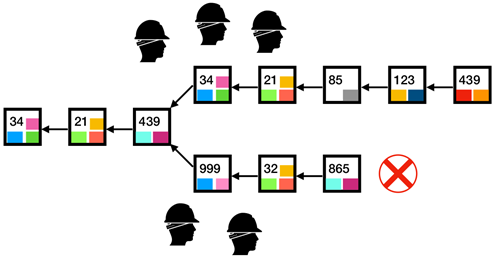
\includegraphics[width=0.8\textwidth]{./figs/longest-chain.png} 
		\caption{Longest chain fork-choice rule.}		
		\label{fig:longest-chain}
	\end{center}	
\end{figure}

\begin{center}\rule{0.5\linewidth}{0.5pt}\end{center}

\subsection{Byzantine Fault
	Tolerance}\label{section-3-byzantine-fault-tolerance}

\subsubsection{The Byzantine Generals
	Problem}\label{the-byzantine-generals-problem}

The Byzantine Generals Problem is a classic thought experiment in
distributed computing that provides a powerful analogy for the
challenges of achieving consensus in a network where some participants
may be unreliable or malicious. The problem is typically stated as
follows (see also \autoref{fig:generals}):

\begin{itemize}
	\item \textit{A group of Byzantine generals are besieging a city. They must decide whether to attack or retreat. If all loyal generals attack, they
		will be victorious. If all loyal generals retreat, they will be saved.
		However, if some generals attack while others retreat, they will be
		defeated. The generals can only communicate with each other via
		messengers, and some of the generals may be traitors who will try to
		disrupt the plan by sending conflicting messages.}
	
\end{itemize}

\begin{figure}[t]
	%	\vspace{-0.3cm}
	\begin{center}
		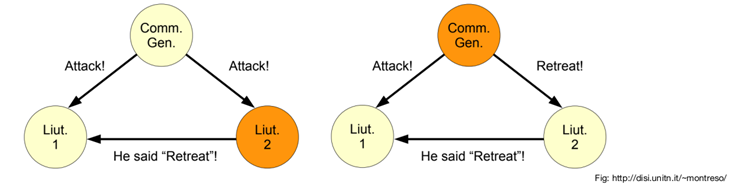
\includegraphics[width=0.9\textwidth]{./figs/byzantyne-generals.png}
		\caption{Byzantine generals problem.}		
		\label{fig:generals}
	\end{center}	
\end{figure}


The problem illustrates the difficulty of achieving consensus in a
distributed system where there is no central authority and where some
nodes may be faulty or malicious. A loyal general receiving conflicting
messages -- for instance, ``attack'' from the commander but ``retreat''
from a fellow lieutenant -- cannot know who the traitor is.

It has been proven that a solution to the Byzantine Generals Problem is
only possible if the number of loyal generals is greater than two-thirds
of the total number of generals. In other words, a system can tolerate
\texttt{f} Byzantine nodes only if the total number of nodes \texttt{N}
is greater than \texttt{3f} (\texttt{f\ \textless{}\ N/3}). This means
that more than two-thirds of the nodes must be honest and follow the
protocol for the system to be able to reach a consensus. This result has
profound implications for the design of fault-tolerant distributed
systems, including blockchains.

\subsubsection{Practical Byzantine Fault Tolerance
	(PBFT)}\label{practical-byzantine-fault-tolerance-pbft}

Practical Byzantine Fault Tolerance (PBFT) \ih{cite} is a landmark consensus
protocol designed to be resilient to Byzantine failures in asynchronous
systems. Developed by Miguel Castro and Barbara Liskov in 1999, PBFT
provides a practical solution to the Byzantine Generals Problem, making
it suitable for use in real-world distributed systems.

PBFT is a voting-based protocol that operates in a series of rounds,
with each round having a designated leader. The protocol involves a
multi-step process to ensure that all honest nodes agree on the order of
operations before they are committed to the ledger. The key phases of
the PBFT protocol are (see also \autoref{fig:pbft}):

\begin{enumerate}
	\def\labelenumi{\arabic{enumi}.}
	\tightlist
	\item
	\textbf{Request}: A client sends a request to the leader node.
	\item
	\textbf{Pre-prepare}: The leader node multicasts the request to all
	other nodes in the network.
	\item
	\textbf{Prepare}: Upon receiving the pre-prepare message, each node
	verifies the request and, if it is valid, multicasts a prepare message
	to all other nodes.
	\item
	\textbf{Commit}: A node waits until it has received \texttt{2f}
	prepare messages from different nodes that match the pre-prepare
	message. At this point, the node multicasts a commit message to all
	other nodes.
	\item
	\textbf{Reply}: A node waits until it has received \texttt{2f\ +\ 1}
	commit messages from different nodes. At this point, the node executes
	the request and sends a reply to the client.
\end{enumerate}

The client waits for \texttt{f\ +\ 1} replies from different nodes with
the same result. This ensures that the result is valid, as at most
\texttt{f} nodes can be malicious.

PBFT is well-suited for permissioned blockchains where the number of
participants is relatively small, due to its $O(N^2)$ communication
complexity. Its ability to provide low-latency finality makes it an
attractive choice for enterprise applications that require high
performance and strong consistency guarantees.

\begin{figure}[t]
	%	\vspace{-0.3cm}
	\begin{center}
		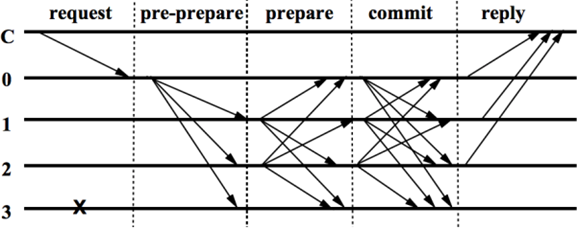
\includegraphics[width=0.75\textwidth]{./figs/pbft.png}
		\caption{Practical Byzantine Fault Tolerant protocol.}		
		\label{fig:pbft}
	\end{center}	
\end{figure}

\begin{center}\rule{0.5\linewidth}{0.5pt}\end{center}

\subsection{Section 4: Consensus Protocols in
	Practice}\label{section-4-consensus-protocols-in-practice}

\subsubsection{Proof-of-Work (PoW)}\label{sec:proof-of-work-pow}

Proof-of-Work (PoW) is the pioneering consensus mechanism that was first
introduced with Bitcoin~\cite{nakamoto2008bitcoin}. It is a permissionless, lottery-based protocol
that allows a decentralized network to reach a consensus without relying
on a central authority.

In a PoW system, nodes, known as miners, compete to solve a
computationally intensive puzzle. This puzzle involves finding a value,
called a nonce, which, when combined with the data in the block and
hashed, produces a hash that is below a certain target value. The
difficulty of this puzzle is adjusted periodically to ensure that a new
block is created at a relatively constant rate (approximately every 10
minutes for Bitcoin), regardless of the total computational power of the
network.

The first miner to find a valid nonce is rewarded with a certain amount
of cryptocurrency, known as the block reward, as well as the transaction
fees from the transactions included in the block. This economic
incentive motivates miners to contribute their computational resources
to the network, thereby securing the blockchain.

PoW is highly scalable in terms of the number of participating nodes, as
anyone can become a miner by simply dedicating computational resources
to the network. However, it has been widely criticized for its high
energy consumption, as the mining process requires a vast amount of
electricity, comparable to that of entire countries. This has led to the
development of alternative consensus mechanisms, such as Proof-of-Stake,
which are more energy-efficient.

\subsubsection{Proof-of-Stake (PoS)}\label{proof-of-stake-pos}

Proof-of-Stake (PoS) is a class of consensus mechanisms that has emerged
as a more energy-efficient alternative to Proof-of-Work. In a PoS
system, the right to create a new block is not determined by a
computational race, but by the amount of cryptocurrency that a node
holds and is willing to ``stake'' as collateral.

The fundamental principle of PoS is that nodes with a larger stake have
a higher probability of being selected to create the next block. This is
because they have a greater vested interest in the security and
integrity of the network. If a validator attempts to add a fraudulent
block to the chain, they risk losing their stake (a process known as
``slashing''), which serves as a powerful economic disincentive against
malicious behavior.

PoS offers several advantages over PoW, including improved energy
efficiency, lower barriers to entry for validators, and the ability to
achieve faster finality. However, it also introduces new challenges,
such as the ``nothing at stake'' problem, where validators have an
incentive to vote for multiple conflicting chains, and the potential for
centralization if a small number of entities accumulate a large portion
of the stake \ih{ref on later}.

\subsubsection{Proof-of-Authority
	(PoA)}\label{proof-of-authority-poa}

Proof-of-Authority (PoA) is a reputation-based consensus mechanism that
is designed for permissioned blockchains. In a PoA network, new nodes
must be approved by a central or federated authority to become
validators. Instead of staking computational resources or
cryptocurrency, validators in a PoA network stake their reputation.

The core idea behind PoA is that validators are incentivized to act
honestly to maintain their reputation. If a validator is found to be
malicious, they can be removed from the network, and their reputation
will be tarnished. This makes PoA a suitable choice for private or
consortium blockchains where the participants are known and trusted
entities, such as a group of financial institutions or a consortium of
universities.

PoA offers several advantages over other consensus mechanisms, including
high throughput, low transaction costs, and energy efficiency. However,
it is also more centralized than permissionless consensus mechanisms
like PoW and PoS, as the authority to validate transactions is
concentrated in a small group of approved nodes.

\begin{center}\rule{0.5\linewidth}{0.5pt}\end{center}


\subsection{Incentive Schemes and Decentralized
	Identities}\label{section-5-incentive-schemes-and-decentralized-identities}

%\subsubsection{Incentive Schemes}\label{incentive-schemes}

Incentive schemes are a critical component of permissionless and
semi-permissionless blockchains, as they provide the economic motivation
for nodes to participate in the consensus process and act honestly.
These schemes typically consist of two main components:

\begin{itemize}
	\tightlist
	\item
	\textbf{Block Rewards}: These are newly created units of
	cryptocurrency that are awarded to the node that successfully creates
	a new block. Block rewards serve as the primary incentive for miners
	in a PoW system and validators in a PoS system.
	\item
	\textbf{Transaction Fees}: These are small fees that are paid by users
	to have their transactions included in a block. Transaction fees
	provide an additional incentive for consensus nodes and become
	increasingly important as the block reward diminishes over time.
	Moreover, transaction fees create the market for the speed of inclusion of transactions in the blockchains -- the higher the fee, the faster inclusion of transaction.
\end{itemize}

The design of the incentive scheme is crucial for the security and
stability of the blockchain. Misaligned incentives can create
vulnerabilities that can be exploited by attackers. For example, if the
transaction fees are too low, miners may be incentivized to create empty
blocks, which can reduce the overall utility of the network.

\subsubsection{Decentralized Names \&
	Identities}\label{decentralized-names-identities}

The management of names and identities in a decentralized system
presents a unique set of challenges. In a traditional centralized
system, a central authority is responsible for managing identities and
ensuring that names are unique. In a decentralized system, however,
there is no such authority, which can lead to problems such as name
collisions and Sybil attacks.

\medskip
\textbf{Zooko's Triangle} is a well-known conjecture in computer science
that illustrates the trade-off among three desirable properties of a
naming system:

\begin{itemize}
	\tightlist
	\item
	\textbf{Human-meaningful}: The names should be easy for humans to
	remember and use (e.g., ``google.com'').
	\item
	\textbf{Secure}: The names should be resistant to spoofing and other
	forms of attack, meaning a name correctly resolves to its intended
	entity.
	\item
	\textbf{Decentralized}: The system should not rely on a central
	authority for name resolution.
\end{itemize}

\begin{figure}[t]
	%	\vspace{-0.3cm}
	\begin{center}
		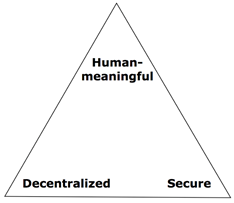
\includegraphics[width=0.3\textwidth]{./figs/zooko.png}
		\caption{Zooko's triangle.}		
		\label{fig:zooko}
	\end{center}	
\end{figure}

Zooko's Triangle posits that it is difficult to achieve all three of
these properties simultaneously. For example, DNS is human-meaningful
and secure (with DNSSec) but centralized. Onion addresses in Tor are
secure and decentralized but not human-meaningful. It is believed that
blockchain technology can help to relax this trade-off by providing a
secure and decentralized platform for managing names and identities.

\textbf{Namecoin} was one of the first projects to attempt to create a
decentralized naming system on a blockchain. It is a fork of Bitcoin
that allows users to register key-value pairs in a censorship-resistant
manner, creating a decentralized domain name system (DNS) with the
top-level domain \texttt{.bit}. However, Namecoin has been plagued by
problems such as \textbf{cyber-squatting} (where users register names
they do not own with the intention of selling them) and
\textbf{front-running} (where an attacker sees a registration
transaction and quickly submits their own for the same name with a
higher fee).

\begin{center}\rule{0.5\linewidth}{0.5pt}\end{center}

\subsection{Summary / Key Takeaways}\label{summary-key-takeaways}

This section has provided a brief exploration of consensus
protocols, the foundational mechanisms that enable the secure and
reliable operation of blockchain networks. We have examined the key
concepts and trade-offs that underpin the design of these protocols,
including:

\begin{itemize}
	\tightlist
	\item
	\textbf{Types of Blockchains}: We have distinguished between
	permissionless, permissioned, and semi-permissionless blockchains,
	highlighting the different access control models and their
	implications for security and decentralization.
	\item
	\textbf{The CAP Theorem}: We have explored the fundamental trade-off
	between consistency, availability, and partition tolerance in
	distributed systems, and how this theorem shapes the design of
	blockchain protocols, leading to eventual consistency.
	\item
	\textbf{Goals of Consensus}: We have defined the key properties of a
	robust consensus protocol: safety, liveness, and finality.
	\item
	\textbf{Lottery vs.~Voting}: We have contrasted the two primary
	approaches to achieving consensus, analyzing their respective
	advantages and disadvantages in terms of scalability, network
	overhead, and time to finality.
	\item
	\textbf{Byzantine Fault Tolerance}: We have delved into the classic
	Byzantine Generals Problem and its solution in the form of Byzantine
	Fault Tolerance, which is essential for building systems that are
	resilient to malicious actors, requiring
	\texttt{N\ \textgreater{}\ 3f} nodes.
	\item
	\textbf{Consensus in Practice}: We have examined the most prominent
	consensus protocols used in real-world blockchains, including
	Proof-of-Work, Proof-of-Stake, and Proof-of-Authority.
	\item
	\textbf{Incentive Schemes and Decentralized Identities}: We have
	discussed the importance of economic incentives in securing blockchain
	networks and the challenges of managing names and identities in a
	decentralized environment, as illustrated by Zooko's Triangle.
\end{itemize}

\begin{center}\rule{0.5\linewidth}{0.5pt}\end{center}

\subsection{Keywords}\label{keywords}

\begin{itemize}
	\tightlist
	\item
	\textbf{Consensus Protocol}: A set of rules and procedures that
	enables a distributed network of computers to achieve agreement on a
	single version of the truth, even in the presence of faults or
	malicious actors.
	\item
	\textbf{Permissionless Blockchain}: A type of blockchain that allows
	anyone to join the network and participate in the consensus process
	without requiring permission from a central authority.
	\item
	\textbf{Permissioned Blockchain}: A type of blockchain that restricts
	access to a limited set of participants who have been granted
	permission to join the network.
	\item
	\textbf{CAP Theorem}: A fundamental theorem in distributed computing
	that states that it is impossible for a distributed data store to
	simultaneously provide more than two of the following three
	guarantees: consistency, availability, and partition tolerance.
	\item
	\textbf{Byzantine Fault Tolerance (BFT)}: The property of a system
	that allows it to tolerate a certain number of faulty or malicious
	nodes (\texttt{f}) without compromising the overall integrity of the
	system, typically requiring more than two-thirds of the nodes to be
	honest (\texttt{N\ \textgreater{}\ 3f}).
	\item
	\textbf{Proof-of-Work (PoW)}: A consensus mechanism that requires
	participants (miners) to solve a computationally intensive puzzle to
	create new blocks, thereby securing the network through the
	expenditure of computational resources.
	\item
	\textbf{Proof-of-Stake (PoS)}: A consensus mechanism in which
	participants (validators) are chosen to create new blocks based on the
	amount of cryptocurrency they hold and are willing to ``stake'' as
	collateral.
	\item
	\textbf{Proof-of-Authority (PoA)}: A consensus mechanism that relies
	on the reputation of a set of pre-approved validators to create new
	blocks, making it suitable for permissioned blockchains.
	\item
	\textbf{Fork}: A situation where a blockchain diverges into two or
	more competing chains.
	\item
	\textbf{Finality}: The property of a consensus protocol that
	guarantees that a transaction, once confirmed, cannot be reversed or
	altered.
	\item
	\textbf{Incentive Scheme}: A set of rules that defines how
	participants in a blockchain network are rewarded (e.g., with block
	rewards and transaction fees) for their contributions to the consensus
	process.
	\item
	\textbf{Zooko's Triangle}: A conjecture that describes the trade-off
	between human-meaningful, secure, and decentralized names in a naming
	system.
\end{itemize}

\begin{center}\rule{0.5\linewidth}{0.5pt}\end{center}

\subsection{Further Reading}\label{further-reading}

\begin{itemize}
	\tightlist
	\item
	\textbf{The Byzantine Generals Problem}:\\
	\url{https://lamport.azurewebsites.net/pubs/byz.pdf}
	\item
	\textbf{Practical Byzantine Fault Tolerance}:\\
	\url{http://pmg.csail.mit.edu/papers/osdi99.pdf}
\end{itemize}

